
\begin{figure}[H]
    \centering
    
\tikzset{every picture/.style={line width=0.75pt}} %set default line width to 0.75pt        

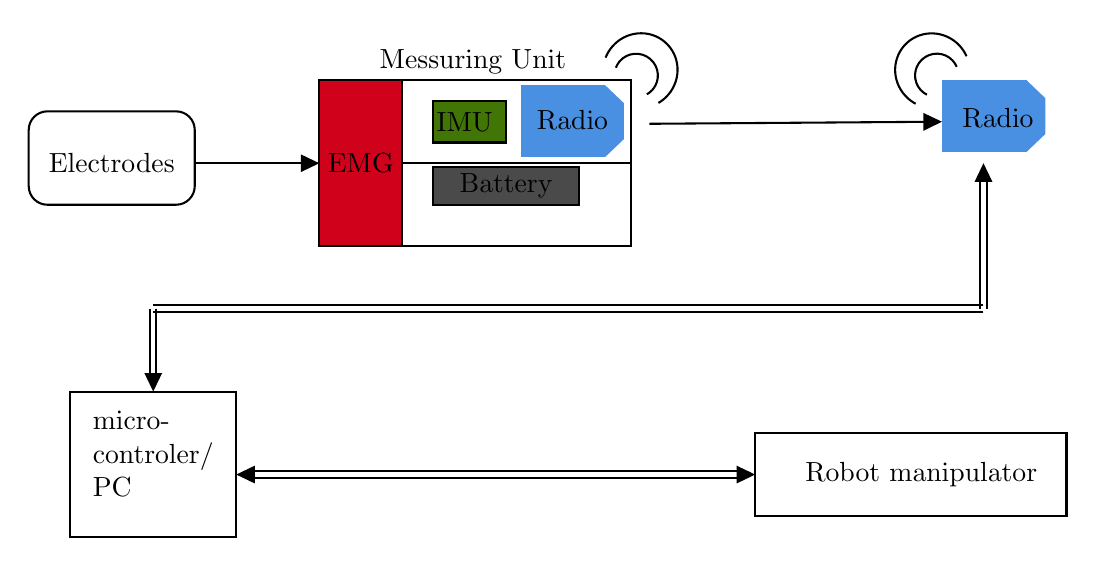
\begin{tikzpicture}[x=0.75pt,y=0.75pt,yscale=-1,xscale=1]
%uncomment if require: \path (0,278.7142848968506); %set diagram left start at 0, and has height of 278.7142848968506

%Rounded Rect [id:dp6413063332380855] 
\draw   (20,54) .. controls (20,49.03) and (24.03,45) .. (29,45) -- (91,45) .. controls (95.97,45) and (100,49.03) .. (100,54) -- (100,81) .. controls (100,85.97) and (95.97,90) .. (91,90) -- (29,90) .. controls (24.03,90) and (20,85.97) .. (20,81) -- cycle ;
%Straight Lines [id:da6300227835642365] 
\draw    (100,70) -- (158,70) ;
\draw [shift={(160,70)}, rotate = 540] [fill={rgb, 255:red, 0; green, 0; blue, 0 }  ][line width=0.75]  [draw opacity=0] (8.93,-4.29) -- (0,0) -- (8.93,4.29) -- cycle    ;

%Shape: Rectangle [id:dp29756334080248226] 
\draw   (160,30) -- (310,30) -- (310,110) -- (160,110) -- cycle ;
%Shape: Rectangle [id:dp330906364121774] 
\draw  [fill={rgb, 255:red, 208; green, 2; blue, 27 }  ,fill opacity=1 ] (160,30) -- (200,30) -- (200,110) -- (160,110) -- cycle ;
%Straight Lines [id:da029037017732416848] 
\draw    (319,51) -- (458,50.01) ;
\draw [shift={(460,50)}, rotate = 539.5899999999999] [fill={rgb, 255:red, 0; green, 0; blue, 0 }  ][line width=0.75]  [draw opacity=0] (8.93,-4.29) -- (0,0) -- (8.93,4.29) -- cycle    ;

%Shape: Rectangle [id:dp532013176046509] 
\draw   (200,30) -- (310,30) -- (310,70) -- (200,70) -- cycle ;
%Shape: Rectangle [id:dp7726211268757011] 
\draw   (200,70) -- (310,70) -- (310,110) -- (200,110) -- cycle ;
%Shape: Diagonal Stripe [id:dp8385620342618032] 
\draw  [color={rgb, 255:red, 0; green, 0; blue, 0 }  ,draw opacity=0 ][fill={rgb, 255:red, 74; green, 144; blue, 226 }  ,fill opacity=1 ] (306.79,58.36) -- (297.73,67) -- (297.73,32.43) -- (306.79,41.07) -- cycle ;
%Shape: Rectangle [id:dp048225570012627283] 
\draw  [draw opacity=0][fill={rgb, 255:red, 74; green, 144; blue, 226 }  ,fill opacity=1 ] (257,32.43) -- (297.73,32.43) -- (297.73,67) -- (257,67) -- cycle ;

%Shape: Rectangle [id:dp24678180631621505] 
\draw  [fill={rgb, 255:red, 74; green, 74; blue, 74 }  ,fill opacity=1 ] (215,72) -- (285,72) -- (285,90) -- (215,90) -- cycle ;
%Shape: Rectangle [id:dp08589280624389195] 
\draw  [fill={rgb, 255:red, 65; green, 117; blue, 5 }  ,fill opacity=1 ] (215,40) -- (250,40) -- (250,60) -- (215,60) -- cycle ;
%Shape: Arc [id:dp5045652470541955] 
\draw  [draw opacity=0] (302.89,23.99) .. controls (303.31,22.88) and (303.92,21.82) .. (304.74,20.86) .. controls (308.48,16.5) and (315.08,16.02) .. (319.46,19.79) .. controls (323.85,23.55) and (324.37,30.14) .. (320.63,34.5) .. controls (319.81,35.46) and (318.86,36.23) .. (317.82,36.8) -- (312.69,27.68) -- cycle ; \draw   (302.89,23.99) .. controls (303.31,22.88) and (303.92,21.82) .. (304.74,20.86) .. controls (308.48,16.5) and (315.08,16.02) .. (319.46,19.79) .. controls (323.85,23.55) and (324.37,30.14) .. (320.63,34.5) .. controls (319.81,35.46) and (318.86,36.23) .. (317.82,36.8) ;
%Shape: Arc [id:dp8674617821007324] 
\draw  [draw opacity=0] (297.95,19.11) .. controls (298.69,17.23) and (299.75,15.44) .. (301.14,13.82) .. controls (307.69,6.19) and (319.05,5.19) .. (326.5,11.59) .. controls (333.96,17.98) and (334.69,29.36) .. (328.14,36.99) .. controls (326.75,38.61) and (325.14,39.94) .. (323.39,40.95) -- (314.64,25.4) -- cycle ; \draw   (297.95,19.11) .. controls (298.69,17.23) and (299.75,15.44) .. (301.14,13.82) .. controls (307.69,6.19) and (319.05,5.19) .. (326.5,11.59) .. controls (333.96,17.98) and (334.69,29.36) .. (328.14,36.99) .. controls (326.75,38.61) and (325.14,39.94) .. (323.39,40.95) ;

%Shape: Arc [id:dp6395313948687686] 
\draw  [draw opacity=0] (452.73,36.97) .. controls (451.67,36.44) and (450.68,35.71) .. (449.82,34.79) .. controls (445.9,30.59) and (446.15,23.98) .. (450.38,20.04) .. controls (454.61,16.09) and (461.21,16.3) .. (465.13,20.5) .. controls (465.99,21.42) and (466.65,22.46) .. (467.11,23.55) -- (457.48,27.65) -- cycle ; \draw   (452.73,36.97) .. controls (451.67,36.44) and (450.68,35.71) .. (449.82,34.79) .. controls (445.9,30.59) and (446.15,23.98) .. (450.38,20.04) .. controls (454.61,16.09) and (461.21,16.3) .. (465.13,20.5) .. controls (465.99,21.42) and (466.65,22.46) .. (467.11,23.55) ;
%Shape: Arc [id:dp6559945001551593] 
\draw  [draw opacity=0] (447.33,41.35) .. controls (445.55,40.4) and (443.88,39.15) .. (442.42,37.58) .. controls (435.56,30.23) and (435.82,18.84) .. (443.01,12.13) .. controls (450.19,5.43) and (461.58,5.96) .. (468.44,13.31) .. controls (469.9,14.88) and (471.03,16.63) .. (471.85,18.47) -- (455.43,25.45) -- cycle ; \draw   (447.33,41.35) .. controls (445.55,40.4) and (443.88,39.15) .. (442.42,37.58) .. controls (435.56,30.23) and (435.82,18.84) .. (443.01,12.13) .. controls (450.19,5.43) and (461.58,5.96) .. (468.44,13.31) .. controls (469.9,14.88) and (471.03,16.63) .. (471.85,18.47) ;

%Straight Lines [id:da36130723234012985] 
\draw    (481.5,78) -- (481.5,140)(478.5,78) -- (478.5,140) ;

\draw [shift={(480,70)}, rotate = 90] [fill={rgb, 255:red, 0; green, 0; blue, 0 }  ][line width=0.75]  [draw opacity=0] (8.93,-4.29) -- (0,0) -- (8.93,4.29) -- cycle    ;
%Straight Lines [id:da3368128282424796] 
\draw    (480,141.5) -- (80,141.5)(480,138.5) -- (80,138.5) ;


%Straight Lines [id:da6986678551956043] 
\draw    (81.5,140) -- (81.5,172)(78.5,140) -- (78.5,172) ;
\draw [shift={(80,180)}, rotate = 270] [fill={rgb, 255:red, 0; green, 0; blue, 0 }  ][line width=0.75]  [draw opacity=0] (8.93,-4.29) -- (0,0) -- (8.93,4.29) -- cycle    ;

%Straight Lines [id:da17642820100898704] 
\draw    (128,218.5) -- (362,218.5)(128,221.5) -- (362,221.5) ;
\draw [shift={(370,220)}, rotate = 180] [fill={rgb, 255:red, 0; green, 0; blue, 0 }  ][line width=0.75]  [draw opacity=0] (8.93,-4.29) -- (0,0) -- (8.93,4.29) -- cycle    ;
\draw [shift={(120,220)}, rotate = 0] [fill={rgb, 255:red, 0; green, 0; blue, 0 }  ][line width=0.75]  [draw opacity=0] (8.93,-4.29) -- (0,0) -- (8.93,4.29) -- cycle    ;
%Shape: Rectangle [id:dp18164367926693248] 
\draw   (370,200) -- (520,200) -- (520,240) -- (370,240) -- cycle ;
%Shape: Diagonal Stripe [id:dp43939989252487766] 
\draw  [color={rgb, 255:red, 0; green, 0; blue, 0 }  ,draw opacity=0 ][fill={rgb, 255:red, 74; green, 144; blue, 226 }  ,fill opacity=1 ] (509.79,55.93) -- (500.73,64.57) -- (500.73,30) -- (509.79,38.64) -- cycle ;
%Shape: Rectangle [id:dp8507327329990411] 
\draw  [draw opacity=0][fill={rgb, 255:red, 74; green, 144; blue, 226 }  ,fill opacity=1 ] (460,30) -- (500.73,30) -- (500.73,64.57) -- (460,64.57) -- cycle ;
%Shape: Rectangle [id:dp7178522299746128] 
\draw   (40,180) -- (120,180) -- (120,250) -- (40,250) -- cycle ;

% Text Node
\draw (60,70) node  [align=left] {Electrodes};
% Text Node
\draw (234,21) node  [align=left] {Messuring Unit};
% Text Node
\draw (282,49) node  [align=left] {Radio};
% Text Node
\draw (250,81) node  [align=left] {Battery};
% Text Node
\draw (180,70) node  [align=left] {EMG};
% Text Node
\draw (230,50) node  [align=left] {IMU};
% Text Node
\draw (450,220) node  [align=left] {Robot manipulator};
% Text Node
\draw (80,210) node  [align=left] {micro-\\controler/\\PC};
% Text Node
\draw (487,48) node  [align=left] {Radio};


\end{tikzpicture}
\caption{Illustration of the general design solution. Arrows indicates the direction information is send.}
    \label{fig:GenDesign}
\end{figure}